\documentclass[acmtog]{acmart}
\usepackage{graphicx}
\usepackage{subfigure}
\usepackage{natbib}
\usepackage{listings}
\usepackage{bm}
\usepackage{amsmath}
\usepackage{algorithm}
\usepackage{algpseudocode}

\definecolor{blve}{rgb}{0.3372549 , 0.61176471, 0.83921569}
\definecolor{gr33n}{rgb}{0.29019608, 0.7372549, 0.64705882}
\makeatletter
\lst@InstallKeywords k{class}{classstyle}\slshape{classstyle}{}ld
\makeatother
\lstset{language=C++,
	basicstyle=\ttfamily,
	keywordstyle=\color{blve}\ttfamily,
	stringstyle=\color{red}\ttfamily,
	commentstyle=\color{magenta}\ttfamily,
	morecomment=[l][\color{magenta}]{\#},
	classstyle = \bfseries\color{gr33n}, 
	tabsize=2
}
\lstset{basicstyle=\ttfamily}

% Title portion
\title{Final Project:\\ {Liquid Simulation by SPH Method}} 

\author{Name:\quad Aibo Hu, Student Number:\ 2021533147, Email:\quad huab@shanghaitech.edu.cn\\Name:\quad Jiaying Du, Student Number:\ 2021533037, Email:\quad dujy2@shanghaitech.edu.cn}

% Document starts
\begin{document}
\maketitle

\vspace*{2 ex}

\section{Introduction}
\begin{itemize}
	\item Project skeleton. Render particles. (Aibo Hu)
	\item The basic SPH solver (Aibo Hu, Jiaying Du)
	\item The incompressible SPH solver, PCISPH. (Aibo Hu)
	\item CUDA implementation of PCISPH. (Aibo Hu)
	\item Surface extraction for rendering. (Jiaying Du)
\end{itemize}
\section{Implementation Details}

\subsection{Skeleton}
The code of assignment 5 is used as the skeleton of the project.
Because it provides a basic framework such as Phong shading, time system, and OpenGL abstraction.
We add a class called ParticleSystem to manage the particles.
\subsection{SPH}

Smoothed-particle hydrodynamics (SPH) is a computational fluid dynamics (CFD) method used to simulate the motion and interaction of fluids. It is a meshless method, meaning that it does not use a fixed grid to discretize the domain. Instead, it represents the fluid using a set of discrete particles, or "markers," which move and interact with each other based on the fluid's physical properties.

SPH is particularly useful for simulating fluids with complex geometries or boundaries, and it has been applied to a wide range of problems in engineering, astrophysics, and other fields.

One key feature of SPH is that it uses a smoothing kernel function to smooth out the properties of the fluid over a certain distance, known as the smoothing length. This allows SPH to capture the smooth, continuous nature of fluids, while still maintaining the discrete particle representation.

Other important quantities in SPH include the density of the fluid, which is calculated using the smoothing kernel and the mass of the particles, and the pressure of the fluid, which is calculated using the equation of state of the fluid.

\subsubsection{Cubic Kernel}

The cubic kernel is defined as:

\[
	W(r,h) = \frac{8}{\pi h^3} \begin{cases}
		1 - 6(\frac{r}{h})^2 + 6(\frac{r}{h})^3 & \text{if } 0 \leq \frac{r}{h} \leq \frac{1}{2} \\
		2(1-\frac{r}{h})^3                      & \text{if } \frac{1}{2} \leq \frac{r}{h} \leq 1 \\
		0                                       & \text{otherwise}
	\end{cases}
\]

We use the cubic kernel to calculate the density of the fluid.

\subsubsection{Spiky Kernel}

The spiky kernel is defined as:

\[
	W(r,h) = \frac{15}{\pi h^6} \begin{cases}
		(h - r)^3 & \text{if } 0 \leq r \le h \\
		0         & \text{otherwise}
	\end{cases}
\]

We use the spiky kernel to calculate the pressure of the fluid.

\[
	\nabla W(\boldsymbol{r},h) = \frac{45}{\pi h^6} \begin{cases}
		(h - r)^2\frac{\boldsymbol{r}}{r} & \text{if } 0 \leq r \le h \\
		0                                 & \text{otherwise}
	\end{cases}
\]

\subsubsection{Viscosity Kernel}

The viscosity kernel is defined as:

\[
	W\ (\boldsymbol{r},h)=
	\begin{cases}
		\frac{15}{2\pi h^2}\ \left(-\cfrac{r^3}{2h^3}+\cfrac{r^2}{h^2}+\cfrac{h}{2r}-1\right) & , 0\le r\le h     \\
		0                                                                                     & , \text otherwise \\
	\end{cases}
\]

\[
	\Delta W\ (r,h) = \frac{45}{\pi h^6} \begin{cases}
		(h - r) & \text{if } 0 \leq r \le h \\
		0       & \text{otherwise}
	\end{cases}
\]\

\subsection{Calculate physical quantity}

The physical quantity of any particle can be obtained by summing the relevant properties of all the particles that lie within the range of the kernel, the latter being used as a weighting function $W$.

For a given point $\boldsymbol{r}$,
\[A(\boldsymbol{r}) = \int A(\boldsymbol{r'})W(|\boldsymbol{r}-\boldsymbol{r'}|,h)\mathrm{d}V(\boldsymbol{r'})\]
The integral is approximated using a Riemann summation over the particles,
\[A(\boldsymbol{r}) \approx \sum_j \rho_j A_j W(|\boldsymbol{r}-\boldsymbol{r}_j|,h)\]

\subsubsection{Density}
The density of the fluid is calculated using the smoothing kernel and the mass of the particles.
\[
	\rho_i = \sum_{j=1}^N m_j W(|\boldsymbol{x}_i - \boldsymbol{x}_j|, h)
\]
We assume that the mass of each particle is the same, so we can simplify the equation to:
\[
	\rho_i = m \sum_{j=1}^N  W(|\boldsymbol{x}_i - \boldsymbol{x}_j|, h)
\]

\subsection{Particle force}
In smoothed-particle hydrodynamics (SPH), there are several forces that influence the motion and behavior of the fluid. These forces can be broadly classified as external forces and internal forces.

External forces include forces that are applied to the fluid from the outside, such as gravity, surface tension, and body forces. These forces are typically calculated using the mass of the particles and the external field acting on them.

Internal forces include forces that are generated within the fluid itself, such as pressure and viscosity. The pressure force is a force that acts to balance the internal pressure of the fluid with the external forces acting on it. It is calculated using the equation of state of the fluid and the density of the particles. The viscosity force is a force that acts to resist the motion of the fluid and promote mixing. It is calculated using the viscosity kernel and the velocity and density of the particles.

\subsubsection{External force}
The external force is calculated using the mass of the particles and the external field acting on them.
\[
	\boldsymbol{F}^{ext} = \boldsymbol{g} \cdot m
\]
\subsubsection{Viscosity force}
The viscosity force is a force that acts to resist the motion of the fluid and promote mixing. It is calculated using the viscosity kernel and the velocity and density of the particles.
\[
	\boldsymbol{F}^{vis}_i = \sum_j \mu \cdot \frac{m}{\rho_j} \cdot \Delta W(\boldsymbol{r},h) \cdot (\boldsymbol{v}_{j} - \boldsymbol{v}_{i})
\]

where $\mu$ is the viscosity coefficient, $m$ is the mass of the particle, $\rho_j$ is the density of the particle $j$, $\boldsymbol{r}=x_{cur} - x_{other}$ is the vector between two particles, $r=|\boldsymbol{r}|$, and $h$ is the smoothing length.
$\sum_j$ is the summation of all the particles in the neighborhood of the particle $i$.

\subsubsection{Pressure force}
The pressure force is a force that acts to balance the internal pressure of the fluid with the external forces acting on it. It is calculated using the equation of state of the fluid and the density of the particles.
\[
	\boldsymbol{F}^{pre}_i = -m^2 \sum_j (\frac{p_i}{\rho_i} + \frac{p_j}{\rho_j})\nabla W(\boldsymbol{r},h)
\]
where $\boldsymbol{r}=x_{i} - x_{j}$ is the vector between two particles, $r=|\boldsymbol{r}|$, and $h$ is the smoothing length.

\subsubsection{Total force}
The total force is the sum of the external force, the viscosity force, and the pressure force.
\[
	\boldsymbol{F}_i = \boldsymbol{F}^{ext}_i + \boldsymbol{F}^{vis}_i + \boldsymbol{F}^{pre}_i
\]

\subsection{PCISPH}
Predictive-Corrective Incompressible SPH is a method for solving the incompressibility constraint in SPH.
It is based on the idea of using a predictor-corrector scheme to solve the incompressibility constraint.
The predictor step is used to calculate the velocity of the particles, and the corrector step is used to calculate the pressure of the particles.
\subsubsection{Algorithm}

\begin{algorithm}
	\caption{An algorithm with caption}\label{alg:pcisph}
	\begin{algorithmic}
		\While{animating}
		\For{each particle $i$}
		\State compute forces $\boldsymbol{F}^{ext, vis}_i(t)$
		\State initialize pressure $p_i(t)=0$
		\State initialize pressure force $\boldsymbol{F}^p_i(t)=0$
		\EndFor
		\While{$\rho_{err}^*(t+1) > \eta$ || $iter < minIteration$}
		\For{each particle $i$}
		\State predict position $\boldsymbol{x}_i^*(t+1)$
		\EndFor
		\For{each particle $i$}
		\State predict density $\rho_i^*(t+1)$
		\State predict density variation $\rho_{{err}_i}^*(t+1) = \rho_i^*(t+1) - \rho_0$
		\State update pressure $p_i(t) += f(\rho_{{err}_i}^*(t+1))$
		\EndFor
		\For{each particle $i$}
		\State compute pressure force $\boldsymbol{F}^p(t)$
		\EndFor
		\EndWhile
		\For{each particle $i$}
		\State compute new velocity $\boldsymbol{v}_i(t+1)$
		\State compute new position $\boldsymbol{x}_i(t+1)$
		\EndFor
		\EndWhile
	\end{algorithmic}
\end{algorithm}

The PCISPH method is illustrated in Algorithm~\ref{alg:pcisph}

Intuitively, the algorithm guess the pressure force, and then compute the position and density of the particles. Then, it computes the density error and update the pressure. The algorithm iterates until the density error is small enough or the maximum number of iterations is reached.

Let $\tilde{p}_i = f(\rho_{err_i}^*)$.
In the paper, the function $f$ is defined as:
\[
	f(\rho_{err_i}^*) = \delta \rho_{err_i}^*
\]
where
\[
	\delta = \frac{-1}{\beta(\sum_j \nabla W_{ij} \cdot \sum_j \nabla W_{ij} - \sum_j(\nabla W_{ij}\cdot \nabla W_{ij}))}
\]
where $\beta = \Delta t^2 m^2 \frac{2}{\rho_0^2}, W_{ij} = W(\boldsymbol{x}_i(t) - \boldsymbol{x}_j(t), h)$

$\delta$ is precomputed via perfect sampling, and is used to compute the pressure force for every particle.

\subsubsection{CPU implementation}

The CPU implementation is in src/pcisph.cpp. We create a class Particle that contains the position, velocity, density, pressure, and pressure force of a particle.
We also create a class PCISPH that contains the particles and the methods to compute the forces and the pressure.
We use OpenMP to parallelize the algorithm.

\begin{lstlisting}[language=C++,basicstyle=\ttfamily\small]
class Particle {
public:
	Vec3 x{0, 0, 0}, v{0, 0, 0}, a{0, 0, 0};
	Float density = density_0, pressure;
	Vec3 x_pred, pressure_accel;
	std::vector<Particle *> neighbors;
};
class ParticleSystem {
public:
  std::vector<Particle> particles;
  std::vector<Vec3> boundaries;

  robin_hood::unordered_map<int,
    std::vector<Particle *>> grid;
  void buildGrid();

  void pci_sph_solver();
  void advect_non_pressure_force();
  void compute_delta();
  void pressure_iteration();
  void advect_pressure();
  Float delta = 0;
  Float density_err_max = 0;

  void simulate();
  void simulate(unsigned num_steps);
  void fixedUpdate();
};
\end{lstlisting}

\subsection{CUDA implementation}

It is easy to parallelize the PCISPH algorithm using CUDA since every particle is independent from the others.

Implement a hash table and vector on GPU is hard.
So, instead of hash table and variable length vector, we use static array and avoid the use of hash table and vector.

The CUDA implementation is in pcisph/pcisph.cu.

\section{Surface extraction}

In the surface rendering part, I adopted the marchcube method for its simplicity and wide usage.

The marchcube method is a method described below:

When You are processing a cloud of particles you can compute the density of them like in the steps above. Therefore,
you can assume at a sample point there is a particle, you can compute the density of the hypothetical particle.

We figure out the possible space where liquid may appear and we divide the space with mesh cube. We can get sample points lying on
every cross point of the mesh cube. We compute the density for each point. We can get the condition of each small grid.

Having got the condition for each small grid. We set a threshold density and then binarize the values. We can design a map mapping each condition of small grid ($2^8$) to
different surface conditions, i.e. different vertices and different faces. Because the cubes are adjacent we have to design the map carefully.
Therefore I use the universially recogized marching cube map.

Then we can get the vertices and faces of the surface. Drawing them out we get the surface rendering outcome.

\section{Results}

\subsection{PCISPH}

Fig~\ref{fig:particle} shows the results of the simulation.
It is the 90th frame of the simulation
The scene contains 44294 particles.

\begin{figure}[h]
	\centering
	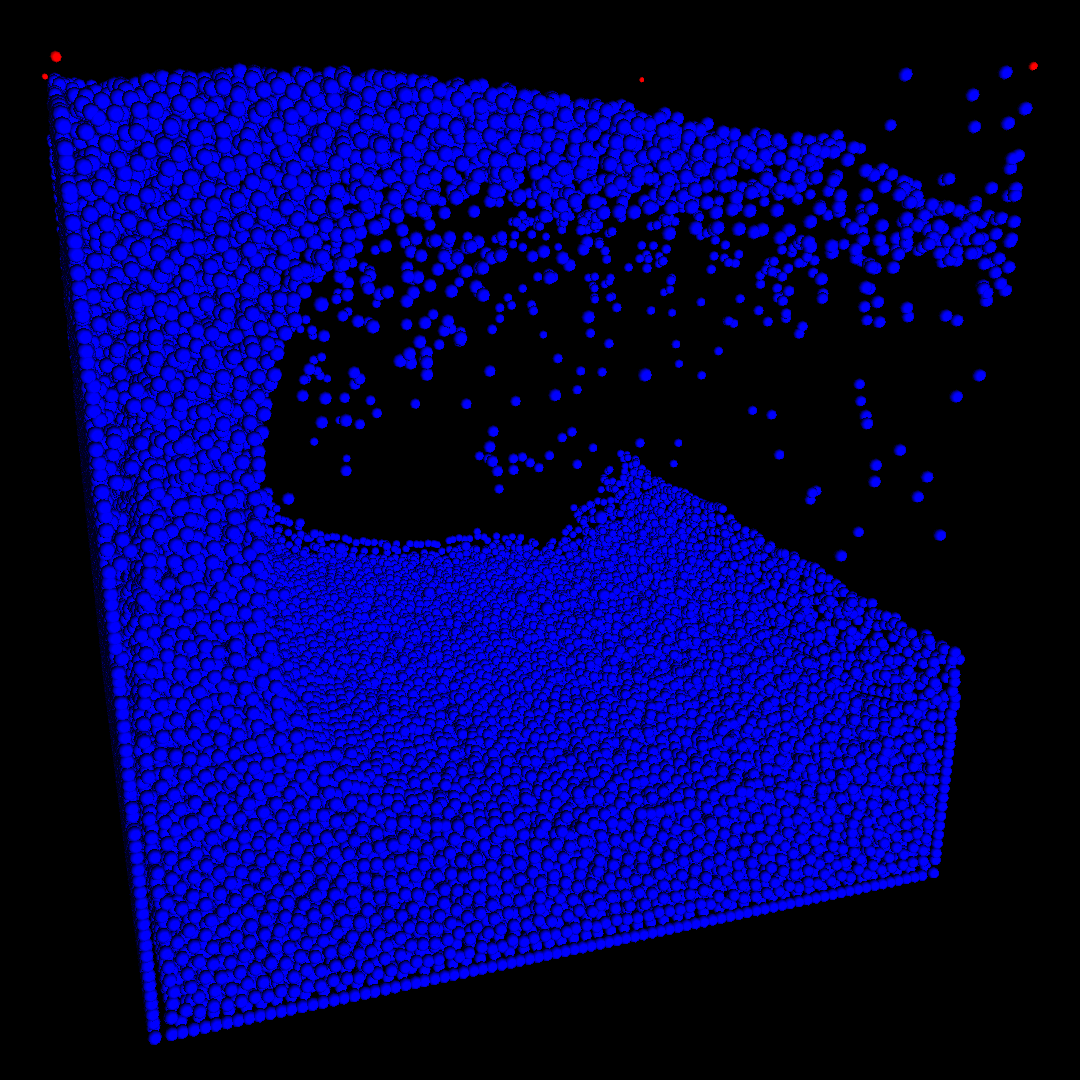
\includegraphics[width=0.40\textwidth]{particle.png}
	\caption{PCISPH simulation, 44294 particles}
	\label{fig:particle}
\end{figure}

\subsection{CUDA}

CUDA speeds up the simulation dramatically.
All timings are given for two EPYC-7742(128 cores in total) or one V100.
The result is shown in Tab~\ref{tab:cuda}

\begin{table}[h]
	\begin{tabular}{l|l|l|l}
		Particles & CPU Time (ms) & CUDA Time (ms) & Speed up \\ \hline
		44294     & 371869        & 3191           & 116.5x   \\ \hline
		9261      & 99038         & 1714           & 57.7x    \\ \hline
		3375      & 33836         & 1716           & 19.71x   \\ \hline
		1331      & 15783         & 1439           & 10.9x    \\ \hline
		343       & 7015          & 1140           & 6.1x     \\
	\end{tabular}
	\caption{CUDA speed up}
	\label{tab:cuda}
\end{table}

\subsection{Surface extraction}

\begin{figure}[h]
	\centering
	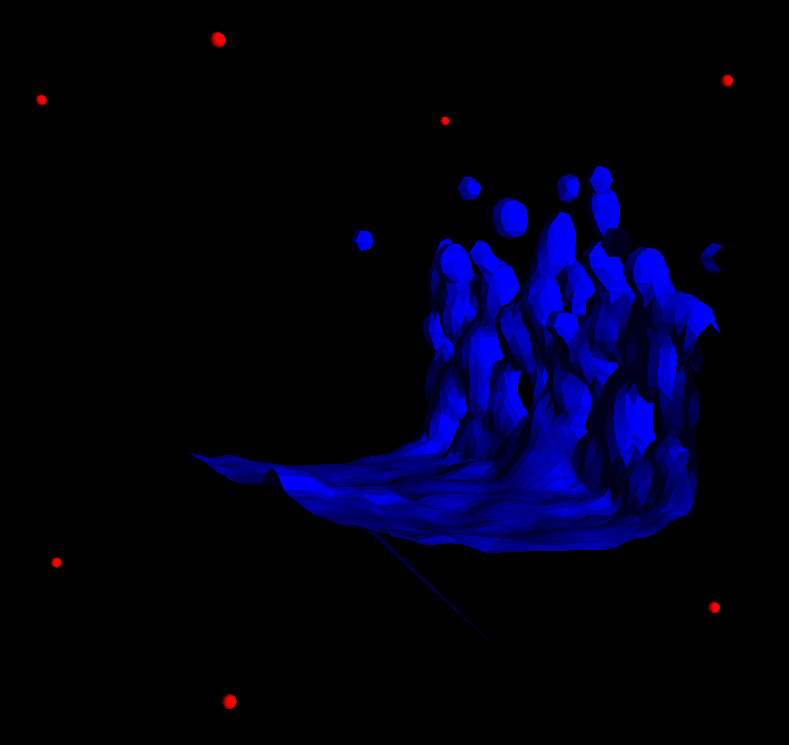
\includegraphics[width=0.40\textwidth]{surface-extraction.png}
	\caption{Surface extraction}
\end{figure}


\end{document}
